\documentclass[12pt,a4paper,oneside]{article} %% Dokumenten Parameter und Art des Dokuments
\usepackage[utf8x]{inputenc} %% Diese Datei ist im utf8 Format dies ist hier damit Latex uns versteht
\usepackage[ngerman]{babel} %% Rechtschreib prüfung
\usepackage{hyperref}
\usepackage{amsmath} %% Packet zur verwendung Mathematischer Formeln
\usepackage{amsfonts}
\usepackage{amssymb} %% Packet zur verwendung Mathematischer Symbole
\usepackage{mathtools}
\usepackage{microtype} %% Sorgt für besseren umgang mit zu lange/kurzen Zeilen
\usepackage{pdfpages} %% Zum einfügen eines PDf dokuments
\title{
	\underline{\underline{Mathematik für die Informatik A, 2018W}} \\
	\underline{\underline{Abgabe zu Blatt N}}
	}
\author{Von: Bennet Bleßmann (stu201758)}

\begin{document}
\maketitle

\setlength{\parindent}{0pt}
\section*{\underline{Aufgabe 1.1}}

\subsection*{a)}

\includegraphics[width=\textwidth]{part/S1A1MA}

\subsection*{b)}

\includegraphics[width=\textwidth]{part/S1A1MB}

\subsection*{c)}

\includegraphics[width=\textwidth]{part/S1A1MASB}
\includegraphics[width=\textwidth]{part/S1A1MAVB}
\includegraphics[width=\textwidth]{part/S1A1MAMB}
\includegraphics[width=\textwidth]{part/S1A1MBMA}

\subsection*{d)}

\includegraphics[width=\textwidth]{part/S1A1MC1}
\includegraphics[width=\textwidth]{part/S1A1MC2}	
\section*{\underline{Aufgabe 1.2}}

\subsection*{a)}

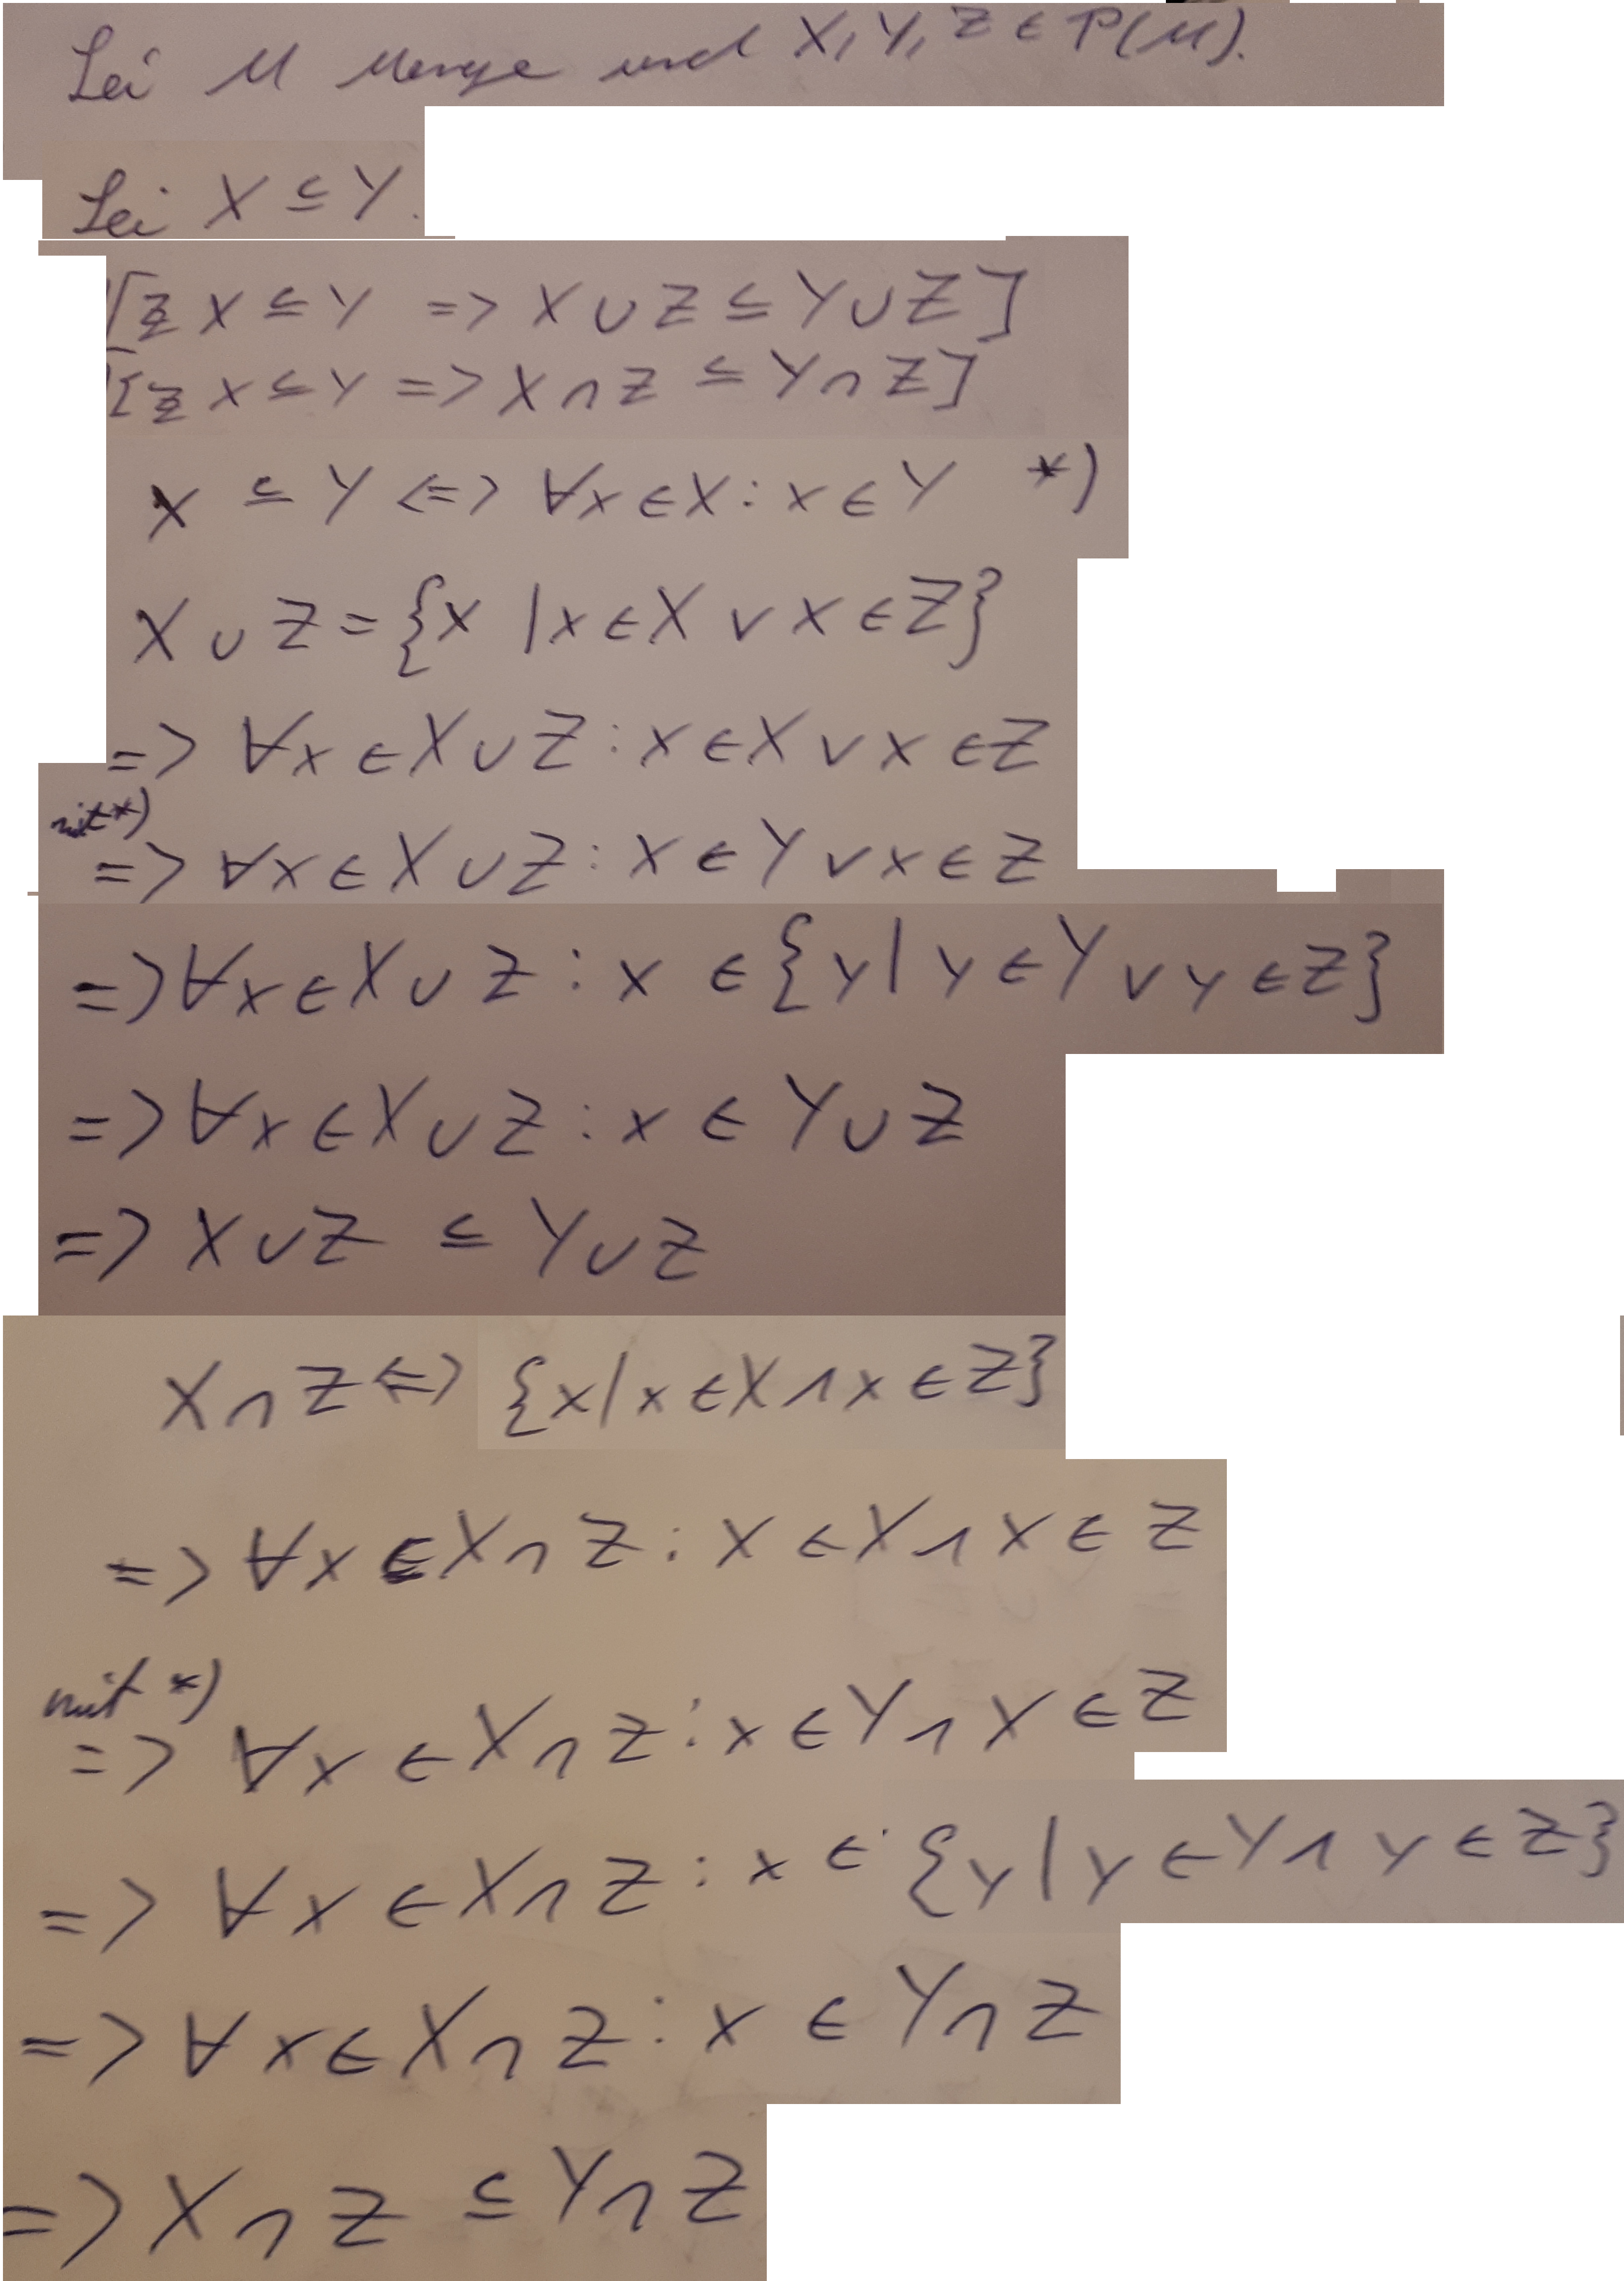
\includegraphics[width=\textwidth]{part/S1A2a}

\subsection*{b)}	
\section*{\underline{Aufgabe N}}

\subsection*{a)}	
\end{document}